\chapter{El corazón y el ciclo cardíaco}\label{ch:b2:heart}

Si se extrae el \omterm{def:b2:heart:anatomy}{corazón} de una rana y se sumerge en una solución salina,
sigue latiendo durante horas --- sin nervios, sin encéfalo, sin \omterm{def:b2:blood-circulation:blood}{sangre},
solo un músculo que se contrae por sí mismo alrededor de una vez por
segundo porque un pequeño grupo de sus células no puede estarse quieto.
Un \omterm{def:b2:heart:anatomy}{corazón} humano lo hace unos tres mil millones de veces a lo largo de
una vida, moviendo del orden de doscientos millones de litros, sin
apagarse nunca. Este capítulo trata de esa bomba: sus cavidades y sus
válvulas, el ciclo de llenado y vaciado y las presiones que lo impulsan,
el sistema eléctrico que lo sincroniza y el trazado que deja en la piel,
la ley que le permite ajustar su gasto a lo que le llega latido a latido,
y los nervios y las hormonas que regulan su ritmo y su fuerza.

\section{La bomba}

\begin{definition}[Cavidades y válvulas]\label{def:b2:heart:anatomy}
\index{corazón}\index{aurícula}\index{ventrículo}\index{válvula cardíaca}
El corazón son dos bombas una junto a otra, cada una formada por una
\emph{aurícula}, que recibe la \omterm{def:b2:blood-circulation:blood}{sangre} de las \omterm{def:b2:blood-circulation:vessels}{venas}, y un
\emph{ventrículo}, que la expulsa a una \omterm{def:b2:blood-circulation:vessels}{arteria}. El corazón derecho recibe
la \omterm{def:b2:blood-circulation:blood}{sangre} de las \omterm{def:b2:blood-circulation:vessels}{venas} cavas y la envía a los pulmones por la \omterm{def:b2:blood-circulation:vessels}{arteria}
pulmonar; el corazón izquierdo la recibe de vuelta por las \omterm{def:b2:blood-circulation:vessels}{venas}
pulmonares y la envía al cuerpo por la aorta. Cuatro válvulas hacen que el
flujo sea unidireccional: las \emph{válvulas auriculoventriculares}
(tricúspide a la derecha, mitral a la izquierda), valvas sujetas por
cuerdas a los músculos papilares para que no puedan ser empujadas hacia la
aurícula; y las \emph{válvulas semilunares} (pulmonar y aórtica), tres
bolsillos que se llenan y cierran cuando la presión arterial supera la del
ventrículo. Las válvulas son pasivas: se abren y se cierran solo por
diferencias de presión. La pared ventricular es el \emph{miocardio},
músculo estriado de células ramificadas unidas extremo con extremo por
\emph{discos intercalares} llenos de uniones comunicantes, de modo que todo
el ventrículo es eléctricamente una sola célula y se contrae como tal; la
pared del ventrículo izquierdo es tres veces más gruesa que la del derecho
porque bombea contra una presión cinco veces mayor. El músculo cardíaco se
nutre por sus propias \emph{\omterm{def:b2:blood-circulation:vessels}{arterias} coronarias}, que se llenan en
diástole, y funciona casi exclusivamente con metabolismo aerobio --- no
puede endeudarse.
\end{definition}

\begin{omfigure}
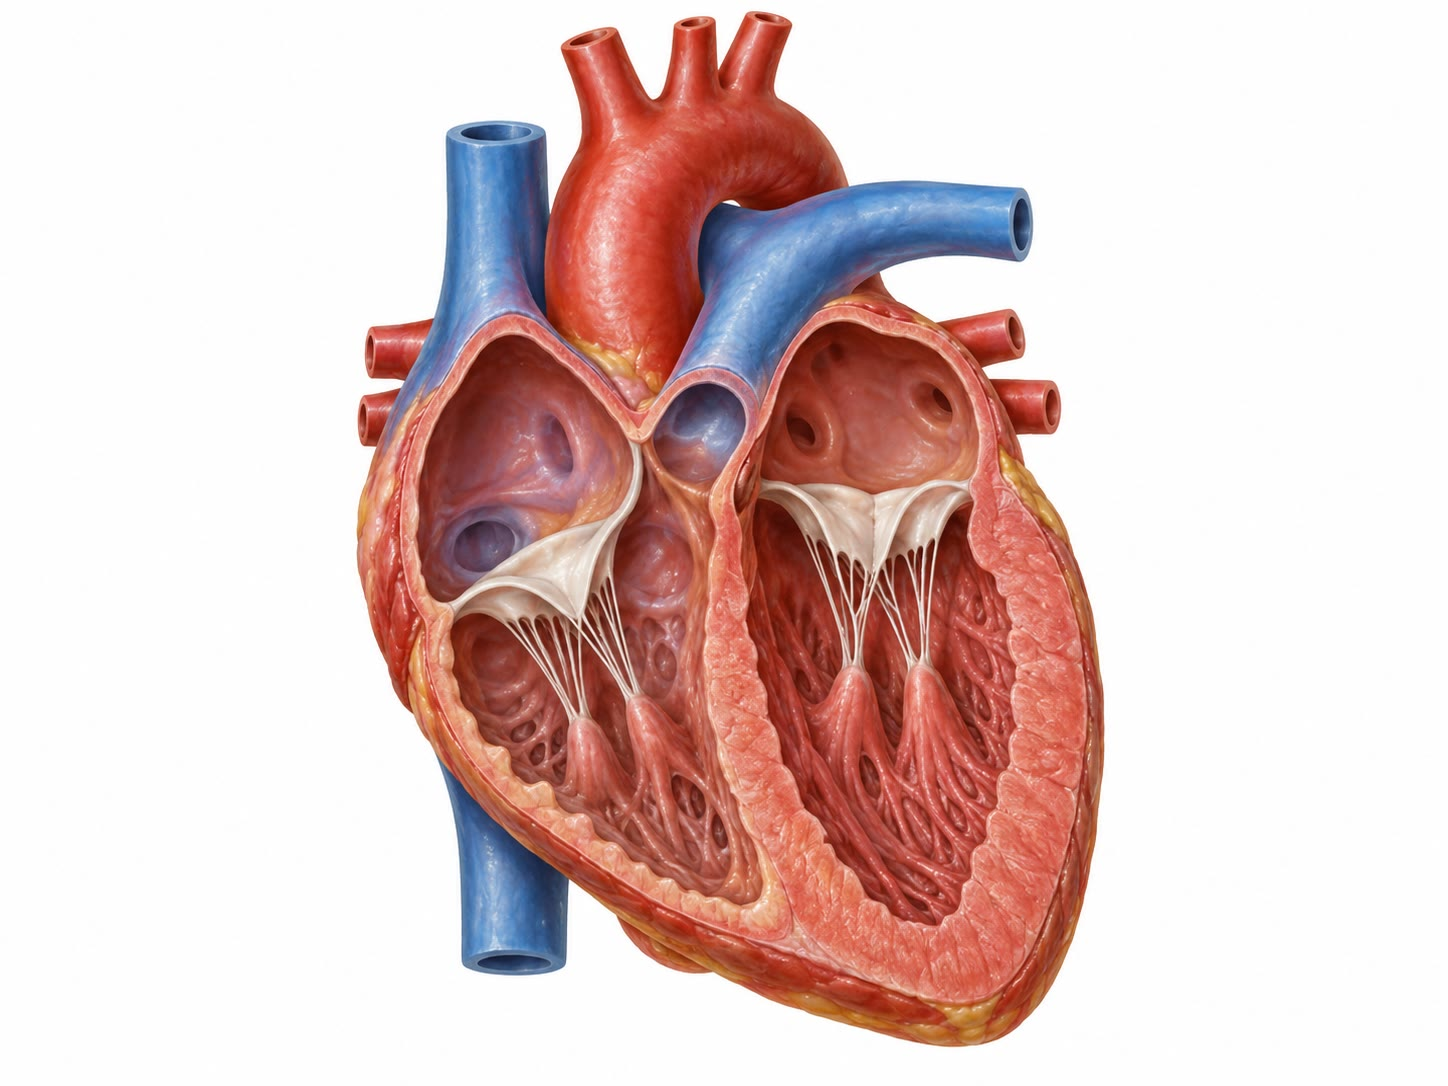
\includegraphics[width=0.55\linewidth]{images/book4/ai/b4-17-heart-cutaway.jpg}

{\small El \omterm{def:b2:heart:anatomy}{corazón} en sección frontal: dos \omterm{def:b2:heart:anatomy}{aurículas} arriba, dos
\omterm{def:b2:heart:anatomy}{ventrículos} abajo, el grueso \omterm{def:b2:heart:anatomy}{ventrículo} izquierdo, las válvulas
auriculoventriculares con sus cuerdas y las dos grandes \omterm{def:b2:blood-circulation:vessels}{arterias} que
salen por arriba.}
\end{omfigure}

\begin{proposition}[El ciclo cardíaco]\label{prop:b2:heart:cycle}
\index{ciclo cardíaco}\index{sístole}\index{diástole}\index{volumen sistólico}\index{fracción de eyección}
Un latido en reposo dura unos \qty{0.8}{s}. \emph{Diástole}
(\qty{0.5}{s}): los \omterm{def:b2:heart:anatomy}{ventrículos} se relajan, su presión cae por debajo de la
de las \omterm{def:b2:heart:anatomy}{aurículas}, las válvulas auriculoventriculares se abren y la \omterm{def:b2:blood-circulation:blood}{sangre}
entra, sobre todo de forma pasiva, y después con un último empujón de la
contracción auricular; el \omterm{def:b2:heart:anatomy}{ventrículo} termina la diástole con unos
\qty{120}{mL} (el \emph{volumen telediastólico}). \emph{Sístole}
(\qty{0.3}{s}): los \omterm{def:b2:heart:anatomy}{ventrículos} se contraen; en cuanto su presión supera la
de las \omterm{def:b2:heart:anatomy}{aurículas}, las válvulas auriculoventriculares se cierran (el primer
ruido cardíaco, ``lub'') y, durante unas centésimas de segundo, el
\omterm{def:b2:heart:anatomy}{ventrículo} comprime una cavidad cerrada --- la \emph{contracción
isovolumétrica} --- hasta que su presión supera la arterial
(\qty{80}{mmHg} a la izquierda), momento en que se abren las válvulas
semilunares y se expulsa la \omterm{def:b2:blood-circulation:blood}{sangre}. El \omterm{def:b2:heart:anatomy}{ventrículo} izquierdo alcanza
\qty{120}{mmHg} y expulsa unos
\qty{70}{mL} (el \emph{\omterm{prop:b2:heart:cycle}{volumen sistólico}}, una \emph{\omterm{prop:b2:heart:cycle}{fracción de
eyección}} del \qty{60}{\%}); al relajarse, su presión cae por debajo de la
de la aorta, la válvula aórtica se cierra de golpe (el segundo ruido,
``dub''), y una relajación isovolumétrica lleva la presión hasta el nivel
auricular, momento en que se reanuda el llenado. El \omterm{def:b2:heart:anatomy}{corazón} derecho hace lo
mismo con la quinta parte de la presión, y expulsa el mismo volumen.
\end{proposition}

\begin{omfigure}
\begin{tikzpicture}
\begin{axis}[
  width=0.9\linewidth, height=7.2cm,
  axis x line=bottom, axis y line=left,
  xmin=0, xmax=0.8, ymin=0, ymax=130,
  xlabel={tiempo en el ciclo (s)}, ylabel={presión (\unit{mmHg})},
  xlabel style={font=\small, at={(axis description cs:0.5,-0.1)}, anchor=north},
  ylabel style={font=\small},
  tick label style={font=\small}, xtick={0,0.1,0.3,0.8}, ytick={0,40,80,120},
  legend style={font=\scriptsize, at={(0.6,0.45)}, anchor=west, draw=none},
  clip=false,
]
% aortic pressure
\addplot[very thick, omThm] coordinates {(0,82) (0.05,80) (0.1,80) (0.12,95) (0.16,115) (0.2,120) (0.25,112) (0.3,100) (0.32,104) (0.34,100) (0.45,94) (0.6,88) (0.8,82)};
\addlegendentry{aorta}
% left ventricular pressure
\addplot[very thick, omDef] coordinates {(0,5) (0.04,8) (0.05,10) (0.08,60) (0.1,80) (0.12,95) (0.16,115) (0.2,120) (0.25,112) (0.3,100) (0.32,60) (0.35,20) (0.38,5) (0.5,3) (0.7,5) (0.75,8) (0.8,5)};
\addlegendentry{ventrículo izquierdo}
% atrial pressure
\addplot[thick, omProp] coordinates {(0,6) (0.03,9) (0.06,6) (0.1,8) (0.15,6) (0.3,7) (0.36,10) (0.4,5) (0.6,6) (0.75,9) (0.8,6)};
\addlegendentry{aurícula izquierda}
\draw[dashed, gray] (axis cs:0.05,0) -- (axis cs:0.05,128); \node[font=\scriptsize, anchor=south, align=center] at (axis cs:0.05,128) {cierre\\mitral};
\draw[dashed, gray] (axis cs:0.1,0) -- (axis cs:0.1,128); \node[font=\scriptsize, anchor=south, align=center] at (axis cs:0.13,128) {apertura\\aórtica};
\draw[dashed, gray] (axis cs:0.31,0) -- (axis cs:0.31,128); \node[font=\scriptsize, anchor=south, align=center] at (axis cs:0.31,128) {cierre\\aórtico};
\draw[dashed, gray] (axis cs:0.38,0) -- (axis cs:0.38,128); \node[font=\scriptsize, anchor=south, align=center] at (axis cs:0.4,128) {apertura\\mitral};
\node[font=\scriptsize] at (axis cs:0.2,45) {sístole};
\node[font=\scriptsize] at (axis cs:0.55,25) {diástole};
\end{axis}
\end{tikzpicture}

{\small Presiones en el \omterm{def:b2:heart:anatomy}{corazón} izquierdo a lo largo de un latido. El
\omterm{def:b2:heart:anatomy}{ventrículo} comprime una cavidad cerrada hasta superar la presión aórtica,
expulsa la \omterm{def:b2:blood-circulation:blood}{sangre} mientras la supera, se relaja hasta caer por debajo de
la presión auricular, y se llena.}
\end{omfigure}

\begin{theorem}[El trabajo del corazón]\label{thm:b2:heart:work}
\index{trabajo cardíaco}\index{bucle presión--volumen}
Representado como presión en función del volumen, un latido del \omterm{def:b2:heart:anatomy}{ventrículo}
izquierdo describe un bucle --- el llenado a lo largo de la parte inferior,
la contracción isovolumétrica subiendo por el lado derecho, la eyección a
lo largo de la parte superior de \qty{120}{mL} a \qty{50}{mL}, la
relajación isovolumétrica bajando por la izquierda ---, y el área del bucle
es el trabajo mecánico del latido:
\[
W = \oint P\,\mathrm{d}V \approx \bar P_{\text{eyección}}\times \text{volumen sistólico} \approx \qty{100}{mmHg}\times\qty{70}{mL} = \qty{0.93}{J}.
\]
A 72 latidos por minuto, el \omterm{def:b2:heart:anatomy}{ventrículo} izquierdo desarrolla alrededor de
\qty{1.1}{W}, y el derecho \qty{0.2}{W}; el metabolismo del \omterm{def:b2:heart:anatomy}{corazón} es de
unos \qty{8}{W}, de modo que su rendimiento mecánico ronda el \qty{15}{\%},
y el resto es calor y el coste de mantener la tensión. Elevar la presión
contra la que bombea el \omterm{def:b2:heart:anatomy}{corazón} (hipertensión, una válvula aórtica
estrechada) eleva en proporción el trabajo por latido, y el músculo se
engrosa en respuesta, como cualquier músculo --- hasta que su riego
coronario ya no puede seguir el ritmo de su masa.
\end{theorem}
\begin{proof}
El trabajo es fuerza por distancia y, para una presión que actúa sobre una
pared móvil, presión por volumen barrido: $\mathrm{d}W = P\,\mathrm{d}V$.
A lo largo de un bucle cerrado, el trabajo neto es el área encerrada (el
llenado a baja presión cuesta poco; la eyección a alta presión devuelve
mucho más). $\qty{100}{mmHg} = \qty{1.33e4}{Pa}$ y $\qty{70}{mL} =
\qty{7e-5}{m^3}$: $1.33\times 10^{4}\times 7\times 10^{-5} =
\qty{0.93}{J}$; por $1.2$ latidos por segundo, \qty{1.1}{W}.
\end{proof}

\begin{omfigure}
\begin{tikzpicture}
\begin{axis}[
  width=0.62\linewidth, height=6cm,
  axis x line=bottom, axis y line=left,
  xmin=0, xmax=150, ymin=0, ymax=140,
  xlabel={volumen del ventrículo izquierdo (\unit{mL})}, ylabel={presión (\unit{mmHg})},
  xlabel style={font=\small, at={(axis description cs:0.5,-0.12)}, anchor=north},
  ylabel style={font=\small},
  tick label style={font=\small}, xtick={0,50,120}, ytick={0,80,120},
  clip=false,
]
\fill[omDef!12] (axis cs:50,5) -- (axis cs:120,8) -- (axis cs:120,80) -- (axis cs:110,115) -- (axis cs:80,122) -- (axis cs:50,100) -- cycle;
\draw[very thick, omDef, ->] (axis cs:50,5) -- (axis cs:120,8);
\draw[very thick, omDef, ->] (axis cs:120,8) -- (axis cs:120,80);
\draw[very thick, omDef, ->] (axis cs:120,80) .. controls (axis cs:110,118) and (axis cs:80,125) .. (axis cs:50,100);
\draw[very thick, omDef, ->] (axis cs:50,100) -- (axis cs:50,5);
\node[font=\scriptsize, anchor=south] at (axis cs:85,11) {llenado};
\node[font=\scriptsize, anchor=west] at (axis cs:122,44) {contracción isovolumétrica};
\node[font=\scriptsize, anchor=south] at (axis cs:85,124) {eyección};
\node[font=\scriptsize, anchor=east] at (axis cs:48,52) {relajación};
\node[font=\scriptsize] at (axis cs:85,60) {área $=$ trabajo, \qty{0.9}{J}};
\end{axis}
\end{tikzpicture}

{\small El \omterm{thm:b2:heart:work}{bucle presión--volumen} del \omterm{def:b2:heart:anatomy}{ventrículo} izquierdo. El área
encerrada es el trabajo de un latido; una presión arterial más alta eleva
la parte superior del bucle y, con ella, el trabajo.}
\end{omfigure}

\section{El reloj propio del corazón}

\begin{proposition}[Automatismo y conducción]\label{prop:b2:heart:conduction}
\index{nódulo sinoauricular}\index{marcapasos}\index{nódulo auriculoventricular}\index{fibras de Purkinje}
El latido se origina en el \emph{\omterm{prop:b2:heart:conduction}{nódulo sinoauricular}}, un grupo de
células musculares especializadas de la pared de la \omterm{def:b2:heart:anatomy}{aurícula} derecha cuyo
potencial de membrana nunca está en reposo: tras cada potencial de acción
asciende lentamente (un \emph{potencial de marcapasos}, impulsado por una
corriente de sodio que se activa a potenciales negativos y por canales de
calcio) hasta alcanzar el umbral y volver a dispararse, unas cien veces
por minuto si se le deja solo. El impulso se propaga por el músculo
auricular, de célula en célula a través de las uniones comunicantes, y las
\omterm{def:b2:heart:anatomy}{aurículas} se contraen; llega al \emph{\omterm{prop:b2:heart:conduction}{nódulo auriculoventricular}}, el único
puente eléctrico entre \omterm{def:b2:heart:anatomy}{aurículas} y \omterm{def:b2:heart:anatomy}{ventrículos}, que conduce despacio y lo
retrasa una décima de segundo --- el tiempo necesario para que las
\omterm{def:b2:heart:anatomy}{aurículas} terminen de llenar los \omterm{def:b2:heart:anatomy}{ventrículos}; después baja a toda
velocidad por el \emph{haz de His} y las \emph{\omterm{prop:b2:heart:conduction}{fibras de Purkinje}}, células
de conducción rápida que lo reparten por todo el músculo ventricular en
\qty{30}{ms}, de modo que los \omterm{def:b2:heart:anatomy}{ventrículos} se contraen desde la punta hacia
arriba, como una unidad, e impulsan la \omterm{def:b2:blood-circulation:blood}{sangre} hacia las válvulas de
salida. Cada parte de este sistema puede marcar el ritmo por sí sola, cada
una más despacio que la anterior (el nódulo a 100, el nódulo AV a 50, las
\omterm{prop:b2:heart:conduction}{fibras de Purkinje} a 30), de modo que, si el nódulo falla, toma el relevo
un centro inferior --- a un ritmo más lento.
\end{proposition}
\begin{proof}[Evidencia]
Un \omterm{def:b2:heart:anatomy}{corazón} aislado, o una tira de tejido sinoauricular, late en una placa
sin nervios; una tira de \omterm{def:b2:heart:anatomy}{ventrículo} también late, pero más despacio.
Enfriar o calentar solo el \omterm{prop:b2:heart:conduction}{nódulo sinoauricular} cambia la frecuencia de
todo el \omterm{def:b2:heart:anatomy}{corazón}; seccionar el haz AV disocia los \omterm{def:b2:heart:anatomy}{ventrículos}, que laten
entonces a su propio ritmo lento mientras las \omterm{def:b2:heart:anatomy}{aurículas} siguen al ritmo
del nódulo (bloqueo cardíaco). El registro de una sola célula del nódulo
muestra la lenta despolarización diastólica que no tiene ninguna célula
muscular ordinaria; bloquear la corriente de marcapasos la ralentiza.
\end{proof}
\begin{omfigure}
\begin{tikzpicture}[every node/.style={font=\scriptsize}, >=stealth]
  % simplified heart outline, scaled up
  \draw[thick, fill=omThm!6] (0,0) .. controls (-4.2,1.3) and (-3.8,5.4) .. (-1.3,5.8) .. controls (0,6.1) and (0.6,5.6) .. (1.3,5.8) .. controls (3.8,5.4) and (4.2,1.3) .. (0,0);
  \draw[thick] (-3.0,3.5) .. controls (-0.8,3.85) and (0.8,3.85) .. (3.0,3.5);
  \draw[thick] (0,3.75) -- (0,0.6);
  \node at (-1.5,4.7) {aurícula derecha}; \node at (1.5,4.7) {aurícula izquierda};
  \node[align=center] at (-1.3,2.55) {ventrículo\\derecho}; \node[align=center] at (1.3,2.55) {ventrículo\\izquierdo};
  % SA node
  \fill[omDef] (-2.5,5.0) circle (0.16); \node[omDef, anchor=east] at (-3.3,5.4) {nódulo SA}; \draw[omDef] (-3.3,5.35) -- (-2.62,5.08);
  \draw[omDef, dashed] (-2.5,5.0) circle (0.45); \draw[omDef, dashed] (-2.5,5.0) circle (0.8);
  % AV node
  \fill[omDef] (-0.25,3.7) circle (0.14); \node[omDef, anchor=west] at (0.15,4.05) {nódulo AV}; \draw[omDef] (0.15,4.05) -- (-0.12,3.78);
  % bundle and Purkinje
  \draw[very thick, omDef] (-0.25,3.6) -- (-0.25,2.1);
  \draw[very thick, omDef] (-0.25,2.1) .. controls (-0.8,1.4) .. (-1.9,1.1);
  \draw[very thick, omDef] (-0.25,2.1) .. controls (0.8,1.4) .. (1.9,1.1);
  \foreach \p in {(-1.9,1.1),(1.9,1.1)} { \draw[omDef] \p -- ++(-0.3,0.6); \draw[omDef] \p -- ++(0.3,0.7); \draw[omDef] \p -- ++(0,0.85); }
  \node[omDef, anchor=west] at (3.4,1.0) {fibras de Purkinje}; \draw[omDef] (3.4,1.0) -- (2.2,1.1);
  \node[omDef, anchor=east] at (-0.45,3.05) {haz de His};
  % timing
  \node[anchor=west, align=left] at (5.6,5.0) {disparo del nódulo SA: $t = 0$\\despolarización auricular: 0--\qty{80}{ms}};
  \node[anchor=west, align=left] at (5.6,3.5) {retraso del nódulo AV: \qty{100}{ms}};
  \node[anchor=west, align=left] at (5.6,1.9) {haz y fibras de Purkinje:\\ventrículos despolarizados\\hacia los \qty{220}{ms}, primero la punta};
\end{tikzpicture}

{\small El sistema de conducción. El \omterm{prop:b2:heart:conduction}{nódulo sinoauricular} se dispara, las
\omterm{def:b2:heart:anatomy}{aurículas} se despolarizan, el \omterm{prop:b2:heart:conduction}{nódulo auriculoventricular} retrasa el
impulso, y el haz y las \omterm{prop:b2:heart:conduction}{fibras de Purkinje} lo reparten por los \omterm{def:b2:heart:anatomy}{ventrículos}
desde la punta hacia arriba.}
\end{omfigure}

\begin{proposition}[El electrocardiograma]\label{prop:b2:heart:ecg}
\index{electrocardiograma}
El \omterm{def:b2:heart:anatomy}{corazón} es una gran masa de células que se despolarizan y repolarizan
en secuencia, y las corrientes que circulan por el cuerpo a su alrededor
pueden registrarse como tensiones de un milivoltio entre electrodos
colocados en las extremidades: el \emph{electrocardiograma}. Sus ondas son
los acontecimientos del sistema de conducción: la \emph{onda P} es la
despolarización auricular; el \emph{intervalo PR}, plano (\qty{0.16}{s}),
es el retraso AV; el \emph{complejo QRS}, agudo y breve (\qty{0.08}{s}), es
la despolarización ventricular --- grande porque la masa ventricular es
grande, breve porque las \omterm{prop:b2:heart:conduction}{fibras de Purkinje} son rápidas; la \emph{onda T}
es la repolarización ventricular. (La repolarización auricular queda
oculta en el QRS.) El trazado informa de la sincronización y de la
conducción, no de la fuerza: un nódulo AV bloqueado alarga el intervalo PR
o disocia P de QRS, una región muerta del \omterm{def:b2:heart:anatomy}{ventrículo} deforma el QRS, una
\omterm{def:b2:heart:anatomy}{aurícula} irregular (fibrilación auricular) sustituye las ondas P por ruido
y hace latir irregularmente los \omterm{def:b2:heart:anatomy}{ventrículos}, y el intervalo entre ondas R
da la frecuencia.
\end{proposition}

\begin{omfigure}
\begin{tikzpicture}
\begin{axis}[
  width=0.9\linewidth, height=5.2cm,
  axis x line=bottom, axis y line=left,
  xmin=0, xmax=1.0, ymin=-0.4, ymax=1.3,
  xlabel={tiempo (s)}, ylabel={mV},
  xlabel style={font=\small, at={(axis description cs:0.5,-0.12)}, anchor=north},
  ylabel style={font=\small},
  tick label style={font=\small}, xtick={0,0.2,0.4,0.6,0.8,1.0}, ytick={0,1},
  clip=false,
]
\addplot[very thick, omDef] coordinates {(0,0) (0.08,0) (0.1,0.05) (0.14,0.15) (0.18,0.05) (0.2,0) (0.28,0) (0.3,-0.1) (0.31,0) (0.33,1.1) (0.35,0) (0.36,-0.25) (0.375,0) (0.5,0) (0.54,0.1) (0.58,0.28) (0.62,0.1) (0.65,0) (0.88,0) (0.9,0.05) (0.94,0.15) (0.98,0.05) (1.0,0)};
\node[font=\scriptsize, anchor=south] at (axis cs:0.14,0.17) {P};
\node[font=\scriptsize, anchor=south] at (axis cs:0.33,1.12) {R};
\node[font=\scriptsize, anchor=north] at (axis cs:0.295,-0.11) {Q};
\node[font=\scriptsize, anchor=north] at (axis cs:0.365,-0.27) {S};
\node[font=\scriptsize, anchor=south] at (axis cs:0.58,0.3) {T};
\draw[<->, gray] (axis cs:0.1,0.45) -- (axis cs:0.3,0.45); \node[font=\scriptsize, anchor=south, gray] at (axis cs:0.2,0.46) {PR \qty{0.16}{s}};
\draw[<->, gray] (axis cs:0.3,0.6) -- (axis cs:0.375,0.6); \node[font=\scriptsize, anchor=west, gray] at (axis cs:0.38,0.6) {QRS \qty{0.08}{s}};
\draw[<->, gray] (axis cs:0.33,1.25) -- (axis cs:0.94,1.25); \node[font=\scriptsize, anchor=south, gray] at (axis cs:0.63,1.25) {intervalo R--R $=$ 60/frecuencia};
\end{axis}
\end{tikzpicture}

{\small Un electrocardiograma normal: P (\omterm{def:b2:heart:anatomy}{aurículas}), el retraso PR en el
nódulo AV, QRS (despolarización ventricular), T (repolarización
ventricular).}
\end{omfigure}

\section{La regulación del gasto}

\begin{theorem}[La ley de Frank--Starling]\label{thm:b2:heart:starling}
\index{ley de Frank--Starling}\index{precarga}\index{gasto cardíaco}
La fuerza de una contracción ventricular aumenta con el volumen que llenó
el \omterm{def:b2:heart:anatomy}{ventrículo}: dentro del intervalo de funcionamiento, cuanto más se
estira el \omterm{def:b2:heart:anatomy}{ventrículo} en diástole (la \emph{precarga}), más expulsa en
sístole. El \omterm{def:b2:heart:anatomy}{corazón} bombea, por tanto, latido a latido, todo lo que recibe
--- un aumento del retorno venoso del \qty{20}{\%} se compensa con un
aumento del \omterm{prop:b2:heart:cycle}{volumen sistólico} del \qty{20}{\%} sin intervención de ningún
nervio ni hormona ---, y los dos \omterm{def:b2:heart:anatomy}{ventrículos}, que deben mover el mismo
volumen, se equilibran automáticamente: si el \omterm{def:b2:heart:anatomy}{corazón} derecho envía más
\omterm{def:b2:blood-circulation:blood}{sangre} a los pulmones, el izquierdo recibe más y bombea más. El mecanismo
está en el \omterm{def:b2:cell-differentiation:fibre}{sarcómero}: a las longitudes cortas de un \omterm{def:b2:heart:anatomy}{ventrículo} poco lleno,
los filamentos gruesos y finos se solapan demasiado y la sensibilidad al
calcio es baja; estirarlos hacia la longitud óptima (\qty{2.2}{\micro m})
aumenta a la vez el solapamiento disponible para los puentes cruzados y la
sensibilidad, de modo que el mismo pulso de calcio produce más fuerza. Más
allá del óptimo (un \omterm{def:b2:heart:anatomy}{corazón} sobredistendido e insuficiente), la fuerza
vuelve a disminuir.
\end{theorem}
\begin{proof}[Evidencia]
Frank (1895) registró la presión desarrollada por un \omterm{def:b2:heart:anatomy}{ventrículo} de rana
llenado a distintos volúmenes: la presión máxima aumentaba con el volumen
de llenado hasta un máximo y después disminuía. Starling (1914), con una
preparación corazón--pulmón de perro en la que el retorno venoso y la
resistencia arterial podían fijarse de forma independiente, mostró que
aumentar el retorno aumentaba el gasto latido a latido, y que un aumento
de la resistencia arterial se compensaba, tras unos pocos latidos de
acumulación, con un mayor volumen telediastólico y un gasto restablecido
--- el \omterm{def:b2:heart:anatomy}{ventrículo} responde a una carga estirándose y a un estiramiento
contrayéndose con más fuerza.
\end{proof}

\begin{omfigure}
\begin{tikzpicture}
\begin{axis}[
  width=0.66\linewidth, height=5.4cm,
  axis x line=bottom, axis y line=left,
  xmin=0, xmax=200, ymin=0, ymax=140,
  xlabel={volumen telediastólico (\unit{mL})}, ylabel={volumen sistólico (\unit{mL})},
  xlabel style={font=\small, at={(axis description cs:0.5,-0.13)}, anchor=north},
  ylabel style={font=\small},
  tick label style={font=\small}, xtick={0,50,100,150,200}, ytick={0,50,100},
  legend style={font=\scriptsize, at={(0.5,-0.3)}, anchor=north, draw=none, legend columns=3},
  clip=false,
]
\addplot[very thick, omDef, domain=40:200, samples=60] {130*(1-exp(-(x-40)/70))};
\addlegendentry{normal}
\addplot[very thick, omThm, domain=40:200, samples=60] {130*1.3*(1-exp(-(x-40)/55))};
\addlegendentry{con estimulación simpática}
\addplot[very thick, omExo!70!black, domain=40:200, samples=60] {130*0.5*(1-exp(-(x-40)/90))};
\addlegendentry{corazón insuficiente}
\fill[omDef] (axis cs:120,88) circle (2pt); \node[font=\scriptsize, anchor=south east] at (axis cs:118,90) {reposo};
\end{axis}
\end{tikzpicture}

{\small Curvas de Starling. El \omterm{prop:b2:heart:cycle}{volumen sistólico} aumenta con el llenado;
los nervios simpáticos desplazan la curva hacia arriba (más gasto con el
mismo llenado), y un \omterm{def:b2:heart:anatomy}{corazón} insuficiente la desplaza hacia abajo.}
\end{omfigure}

\begin{proposition}[Nervios y hormonas]\label{prop:b2:heart:control}
\index{sistema nervioso simpático!corazón}\index{nervio vago}\index{adrenalina}\index{gasto cardíaco}
El \omterm{thm:b2:heart:starling}{gasto cardíaco} es la frecuencia cardíaca por el \omterm{prop:b2:heart:cycle}{volumen sistólico}:
\qty{5}{L/min} en reposo y hasta \qty{25}{L/min} en un deportista
entrenado durante el ejercicio. Ambos factores los fijan los nervios
autónomos. El \emph{vago} (parasimpático), que libera acetilcolina sobre
el \omterm{prop:b2:heart:conduction}{nódulo sinoauricular}, ralentiza la deriva del marcapasos y mantiene la
frecuencia en reposo en 70 en lugar de los 100 propios del nódulo; si se
seccionan los vagos, la frecuencia aumenta. Los nervios \emph{simpáticos},
que liberan noradrenalina, y la médula suprarrenal, que libera
\emph{adrenalina} a la \omterm{def:b2:blood-circulation:blood}{sangre}, aceleran la deriva (más latidos), aceleran
la conducción y aumentan la fuerza de contracción con cualquier llenado
(una curva de Starling más empinada, la propiedad llamada
\emph{contractilidad}), al aumentar el calcio que llega a los \omterm{def:b2:cell-differentiation:fibre}{sarcómeros} en
cada latido. En el ejercicio se suelta primero el freno vagal y después se
pisa el acelerador simpático, y una frecuencia de 180 con un \omterm{prop:b2:heart:cycle}{volumen
sistólico} de \qty{140}{mL} da \qty{25}{L/min}; las señales se transmiten a
través de los receptores y segundos mensajeros del
\cref{ch:b2:cell-signalling}, y el conjunto lo gobiernan los centros de
regulación de la presión del \cref{ch:b2:blood-pressure}.
\end{proposition}

\begin{example}[Leer un corazón]\label{ex:b2:heart:reading}
Dos ruidos por latido: lub, el cierre de las válvulas AV al comienzo de la
sístole; dub, el cierre de las válvulas semilunares al final. Un soplo es
un flujo turbulento a través de una válvula estrechada (una estenosis) o
de retorno a través de una que no cierra bien (una insuficiencia): un
soplo entre lub y dub es una válvula mitral insuficiente o una válvula
aórtica estrechada; uno después de dub, una válvula aórtica insuficiente.
Un pulso de 70 con una presión arterial de
$120/80$~mmHg supone un \omterm{prop:b2:heart:cycle}{volumen sistólico} cercano a \qty{70}{mL};
una frecuencia de 40 en un deportista es un gran \omterm{prop:b2:heart:cycle}{volumen sistólico} y un
tono vagal intenso; una frecuencia de 40 con un intervalo PR que se alarga
hasta que se pierde un latido es un nódulo AV enfermo. La fisiología de
este capítulo es lo que un médico oye con un estetoscopio en treinta
segundos.
\end{example}

\section{Ejercicios}

\begin{exercise}[$\star$]\label{exo:b2:heart:1}
Sígase una gota de \omterm{def:b2:blood-circulation:blood}{sangre} desde la \omterm{def:b2:blood-circulation:vessels}{vena} cava hasta la aorta, nombrando por
orden cada cavidad, cada válvula y cada vaso.
\end{exercise}

\begin{exercise}[$\star$]\label{exo:b2:heart:2}
Dense las fases del \omterm{prop:b2:heart:cycle}{ciclo cardíaco} con el estado de cada válvula en cada
fase, y el acontecimiento que causa cada uno de los dos ruidos cardíacos.
\end{exercise}

\begin{exercise}[$\star$]\label{exo:b2:heart:3}
Nómbrense por orden las partes del sistema de conducción, con el tiempo que
tarda el impulso en llegar a cada una y la onda del ECG que produce cada
una.
\end{exercise}

\begin{exercise}[$\star$]\label{exo:b2:heart:4}
Enúnciese la \omterm{thm:b2:heart:starling}{ley de Frank--Starling} y dígase por qué garantiza que los dos
\omterm{def:b2:heart:anatomy}{ventrículos} bombeen el mismo volumen.
\end{exercise}

\begin{exercise}[$\star\star$]\label{exo:b2:heart:5}
Un \omterm{def:b2:heart:anatomy}{corazón} tiene un volumen telediastólico de \qty{130}{mL} y un volumen
telesistólico de \qty{50}{mL} a 70 latidos por minuto. Calcúlense el
\omterm{prop:b2:heart:cycle}{volumen sistólico}, la \omterm{prop:b2:heart:cycle}{fracción de eyección} y el \omterm{thm:b2:heart:starling}{gasto cardíaco}. Un \omterm{def:b2:heart:anatomy}{corazón}
insuficiente tiene \qty{180}{mL} y \qty{120}{mL}: vuélvanse a calcular, y
dígase qué le ha ocurrido a la \omterm{prop:b2:heart:cycle}{fracción de eyección}.
\end{exercise}

\begin{exercise}[$\star\star$]\label{exo:b2:heart:6}
Calcúlese el trabajo de un latido para un \omterm{prop:b2:heart:cycle}{volumen sistólico} de
\qty{70}{mL} a una presión media de eyección de \qty{100}{mmHg}, y la
potencia a 72 latidos por minuto. Vuélvase a calcular para un hipertenso a
\qty{150}{mmHg}. ¿Cuánto oxígeno adicional por minuto necesita el segundo
\omterm{def:b2:heart:anatomy}{corazón}, si el rendimiento mecánico es del \qty{15}{\%} y \qty{1}{mL} de
oxígeno rinde \qty{20}{J}?
\end{exercise}

\begin{exercise}[$\star\star$]\label{exo:b2:heart:7}
En un ECG, las ondas R están separadas \qty{0.5}{s} en un registro y
\qty{1.5}{s} en otro. Dense las frecuencias cardíacas. En un tercero, las
ondas P llegan cada \qty{0.6}{s} y los complejos QRS cada \qty{1.8}{s}, sin
relación fija. ¿Qué ha ocurrido?
\end{exercise}

\begin{exercise}[$\star\star$]\label{exo:b2:heart:8}
El potencial de la célula sinoauricular deriva de \qty{-60}{mV} a un umbral
de \qty{-40}{mV} a \qty{25}{mV/s} antes de cada potencial de acción de
\qty{0.15}{s}. Calcúlense el intervalo entre latidos y la frecuencia. La
acetilcolina reduce la deriva a \qty{18}{mV/s} y el potencial de partida a
\qty{-65}{mV}; la noradrenalina eleva la deriva a \qty{40}{mV/s}.
Calcúlense ambas frecuencias.
\end{exercise}

\begin{exercise}[$\star\star$]\label{exo:b2:heart:9}
Explíquese por qué es necesario el retraso del nódulo AV, qué le ocurriría
al gasto sin él y por qué un nódulo AV lento (un intervalo PR largo) es
inofensivo hasta cierto punto y peligroso más allá.
\end{exercise}

\begin{exercise}[$\star\star\star$]\label{exo:b2:heart:10}
Un deportista tiene en reposo una frecuencia de 45 y un gasto de
\qty{5}{L/min}; durante el ejercicio, una frecuencia de 180 y
\qty{30}{L/min}. Calcúlense los volúmenes sistólicos y dígase qué aportan
la curva de Starling y los nervios simpáticos. ¿Por qué la frecuencia no
puede superar útilmente unos 200?
\end{exercise}

\begin{exercise}[$\star\star\star$]\label{exo:b2:heart:11}
Una válvula aórtica estrechada deja una abertura de \qty{1}{cm^2} en lugar
de \qty{3}{cm^2}. Con la continuidad, calcúlese la velocidad de la \omterm{def:b2:blood-circulation:blood}{sangre}
expulsada a \qty{250}{mL/s} a través de cada una y, con Bernoulli
($\Delta P = \tfrac12\rho v^2$), la presión que el \omterm{def:b2:heart:anatomy}{ventrículo} debe
generar por encima de la presión aórtica en cada caso. ¿Qué hace el
\omterm{def:b2:heart:anatomy}{ventrículo} al respecto, y cuál es el coste final?
\end{exercise}

\begin{exercise}[$\star\star\star$]\label{exo:b2:heart:12}
``El \omterm{def:b2:heart:anatomy}{corazón} es una bomba que se regula a sí misma y que el sistema
nervioso solo ajusta.'' Discútase, distinguiendo lo que aportan el
automatismo, la \omterm{thm:b2:heart:starling}{ley de Frank--Starling} y los nervios autónomos, y lo que
puede y no puede hacer un \omterm{def:b2:heart:anatomy}{corazón} trasplantado, que no tiene nervios.
\end{exercise}

\section{Problema: un corazón bajo carga}

\begin{problem}[{Problema de fin de semana --- un mismo corazón seguido
del reposo al ejercicio y a la enfermedad: se cronometra su ciclo, se
calcula su trabajo, se lee su electrocardiograma, se cuantifican su
respuesta de Starling y su control autónomo y se estima el coste de una
válvula estrechada, hasta llegar al gasto en reposo y durante el
ejercicio, el trabajo por latido y el gradiente a través de la
estenosis}]
\label{pb:b2:heart:1}
Datos: en reposo, frecuencia de 70, volumen telediastólico de
\qty{130}{mL}, telesistólico de \qty{60}{mL}, presión media de eyección de
\qty{100}{mmHg} ($\qty{1}{mmHg} = \qty{133}{Pa}$), presión aórtica de
$120/80$~mmHg. La sístole dura \qty{0.3}{s} a cualquier frecuencia.
Marcapasos: deriva de \qty{-60}{mV} a \qty{-40}{mV}, potencial de acción de
\qty{0.15}{s}. El \omterm{def:b2:heart:anatomy}{corazón} consume \qty{20}{J} por mililitro de oxígeno con
un rendimiento mecánico del \qty{15}{\%}; la \omterm{def:b2:blood-circulation:blood}{sangre} coronaria transporta
\qty{0.2}{mL} de oxígeno por mililitro y el \omterm{def:b2:heart:anatomy}{corazón} extrae el \qty{70}{\%}.
Densidad de la \omterm{def:b2:blood-circulation:blood}{sangre}: \qty{1060}{kg/m^3}.

\medskip
\noindent\textbf{Parte I --- El ciclo en reposo.}
\begin{enumerate}
  \item Calcúlense el \omterm{prop:b2:heart:cycle}{volumen sistólico}, la \omterm{prop:b2:heart:cycle}{fracción de eyección} y el \omterm{thm:b2:heart:starling}{gasto
        cardíaco}.
  \item Calcúlense la duración de un ciclo y la de la diástole.
  \item Calcúlense el ritmo medio de eyección durante la sístole, en
        mililitros por segundo, y la velocidad media a través de una
        válvula aórtica de \qty{3}{cm^2}.
  \item La presión ventricular sube a \qty{1500}{mmHg/s} durante la
        contracción isovolumétrica, de 10 a \qty{80}{mmHg}. ¿Cuánto dura
        esa fase?
  \item Calcúlense el trabajo de un latido y la potencia mecánica del
        \omterm{def:b2:heart:anatomy}{ventrículo} izquierdo.
  \item Calcúlense la potencia total y el consumo de oxígeno del \omterm{def:b2:heart:anatomy}{corazón}
        (ambos \omterm{def:b2:heart:anatomy}{ventrículos}: tómese el derecho como la quinta parte del
        izquierdo).
  \item Calcúlese el flujo sanguíneo coronario necesario para aportar ese
        oxígeno.
\end{enumerate}

\medskip
\noindent\textbf{Parte II --- El marcapasos y el trazado.}
\begin{enumerate}[resume]
  \item ¿Qué velocidad de deriva (\unit{mV/s}) da una frecuencia de 70?
  \item Se secciona el vago: la frecuencia pasa a 100. ¿A qué velocidad de
        deriva corresponde?
  \item Calcúlese la velocidad de deriva para una frecuencia de 180
        durante el ejercicio.
  \item En el ECG en reposo, dese el intervalo R--R, y dígase a qué
        corresponden las ondas P, QRS y T.
  \item El intervalo PR es de \qty{0.16}{s} en reposo. Su duración es
        sobre todo el retraso del nódulo AV: explíquese qué consigue ese
        retraso y por qué una frecuencia de 180 exige que el nódulo también
        se acelere.
  \item El ECG de un paciente muestra complejos QRS cada \qty{1.5}{s} y
        ondas P cada \qty{0.8}{s}, sin relación entre ellos. Diagnostíquese,
        dese la frecuencia ventricular y dígase qué tejido marca el ritmo de
        los \omterm{def:b2:heart:anatomy}{ventrículos}.
\end{enumerate}

\medskip
\noindent\textbf{Parte III --- El ejercicio.}
Durante el ejercicio la frecuencia sube a 180 y los nervios simpáticos
aumentan la contractilidad de modo que el volumen telesistólico cae a
\qty{30}{mL}; el retorno venoso eleva el volumen telediastólico a
\qty{150}{mL}.
\begin{enumerate}[resume]
  \item Calcúlense el \omterm{prop:b2:heart:cycle}{volumen sistólico}, la \omterm{prop:b2:heart:cycle}{fracción de eyección} y el
        gasto.
  \item Calcúlese la duración de la diástole a 180 y explíquese por qué la
        frecuencia no puede subir útilmente mucho más.
  \item Calcúlense la potencia del \omterm{def:b2:heart:anatomy}{ventrículo} izquierdo a una presión media
        de eyección de \qty{120}{mmHg} y el consumo de oxígeno del \omterm{def:b2:heart:anatomy}{corazón}.
  \item Calcúlese el flujo coronario necesario y compárese con el de
        reposo. ¿Por qué le supone un problema el acortamiento de la
        diástole?
  \item Sin los nervios simpáticos (un \omterm{def:b2:heart:anatomy}{corazón} trasplantado), la frecuencia
        solo sube lentamente, por la adrenalina de la \omterm{def:b2:blood-circulation:blood}{sangre}, y la
        contractilidad menos. Predígase el gasto en el primer minuto de
        ejercicio usando solo la ley de Starling con el mismo llenado.
  \item Atribúyase el aumento del gasto del reposo al ejercicio a sus tres
        causas (frecuencia, llenado, contractilidad), en litros por minuto
        cada una.
\end{enumerate}

\medskip
\noindent\textbf{Parte IV --- Una válvula estrechada.}
La válvula aórtica se estrecha hasta \qty{1}{cm^2}.
\begin{enumerate}[resume]
  \item Calcúlese la velocidad de eyección en reposo a través de la válvula
        estrechada.
  \item Con Bernoulli, $\Delta P = \tfrac12\rho v^{2}$, calcúlese la
        presión que el \omterm{def:b2:heart:anatomy}{ventrículo} debe añadir para empujar la \omterm{def:b2:blood-circulation:blood}{sangre} a
        través de ella, en mmHg.
  \item Vuélvanse a calcular ambas durante el ejercicio.
  \item ¿Cuál debe ser la presión máxima del \omterm{def:b2:heart:anatomy}{ventrículo} en cada caso para
        mantener normal la presión aórtica, y en qué factor aumenta su
        trabajo por latido en reposo?
  \item La pared del \omterm{def:b2:heart:anatomy}{ventrículo} se engrosa en respuesta. Explíquese por qué
        esto ayuda y por qué acaba fallando (piénsese en el riego coronario
        y en el llenado diastólico).
  \item Enúnciese el resultado: el gasto en reposo y durante el ejercicio,
        el trabajo por latido en reposo y el gradiente a través de la
        válvula estrechada en reposo y durante el ejercicio.
\end{enumerate}
\end{problem}
